% LaTeX fixture for generating earthquake exposure information

% Standard document class set to landscape
\documentclass[a4paper]{article}

% Extra packages
\usepackage[hmargin=0mm,vmargin=10mm]{geometry}
\usepackage[usenames,dvipsnames]{color}
\usepackage{graphicx}
\usepackage{courier}
\usepackage{colortbl}

% Define background colours for MMI levels
% NOTE (Ole): These must be the same as the colours defiened in city_table.py
\definecolor{I}{RGB}{0,0,255}
\definecolor{II}{RGB}{32,159,255}
\definecolor{III}{RGB}{0,207,255}
\definecolor{IV}{RGB}{85,255,255}
\definecolor{V}{RGB}{170,255,255}
\definecolor{VI}{RGB}{255,240,0}
\definecolor{VII}{RGB}{255,168,0}
\definecolor{VIII}{RGB}{255,112,0}
\definecolor{IX}{RGB}{255,0,0}
\definecolor{X}{RGB}{240,0,240}

% Fixed width coloured cell
% Usage: \cell{color}{text}
\newcommand{\cell}[2]{
  \cellcolor{#1}
  \makebox[1.3cm]{#2}
}

% No page numbering
\pagestyle{empty}

% Begin document in earnest
\begin{document}

% Header
\centerline{\Large \textbf{PROTOTIPE}}
\begin{tabular}{lcr}
    
\includegraphics[width=0.08\textwidth]{bnpb_logo} &
    \raisebox{10mm}{\parbox{0.75\textwidth}{\Huge \centerline{\textbf{Perkiraan Dampak Gempa}}}} &
    
\includegraphics[width=0.08\textwidth]{bmkg_logo}
\end{tabular}


% Earthquake statistics as per BMKG sms
\bigskip
\input{event_statistics.tex}

% MMI legend
\bigskip
\hspace{-6mm} \input{exposure_table.tex}

% Map elements
\bigskip
\begin{tabular}{@{}l@{}l}
  \Large \textbf{Penduduk Paparan} & \\
  \parbox[t]{0.7\textwidth}{
    \vspace{0pt}
    \includegraphics{exposure_map}} &
  \hspace{-10mm}
  \parbox[t]{0.3\textwidth}{
    %\vspace{0pt}
    \vspace{2mm}
    \includegraphics[angle=270,width=0.3\textwidth]{city_legend} \\
    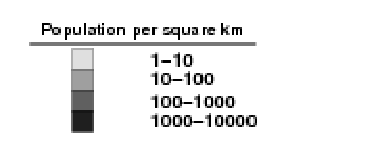
\includegraphics{population_legend}\\
    \includegraphics[width=0.3\textwidth]{mini_map}\\
  }
\end{tabular}

\bigskip
\bigskip
\bigskip

\parbox[t]{0.95\textwidth}{\scriptsize
Pengguna harus mempertimbangkan sifat awal informasi ini dan memeriksa pembaruan sebagai data tambahan telah tersedia. Perkiraan paparan Penduduk TIDAK perkiraan langsung kerusakan gempa; sebanding gemetar akan mengakibatkan kerugian secara signifikan lebih rendah di daerah dengan struktur kekar daripada di daerah dengan struktur rentan. Sambil intensitas dihitung oleh BMKG menggunakan metodologi USGS ShakeMap. Data Penduduk diperkirakan dari Oak Ridge Laboratorys Landscan 2008 Global Penduduk Database. Angka yang dihasilkan menggunakan Python, Generic Mapping Tools (GMT) dan \LaTeX.

Didukung oleh Australia-Indonesia Facility for Disaster Reduction dan Geoscience Australia.}
\end{document}



